\chapter{Revision History}
\label{Chp:RevHistory}
%--------------------------------------------------------------

Changes in 2.0.0 (Released: \#\#-Xxxxx-2021:
\begin{itemize}
\item Reorganized Chapters 2 and 3: Chapter 2 contains prose regarding the basic concepts captured in the API; Chapter 3 presents all of the enumeratiosn, literals, data types, and predefined objects required by the API.  Made short captions for the List of Tables.
\item (Issue BB-49, BB-50) Updated and corrected language regarding multithreading and completion, and requirements regarding acquire-release memory orders.  Methods that used to force complete no longer do.
\item (Issue BB-74, BB-9) Assigned integer values to all return codes as well as all enumerations in the API to ensure run-time compatibility between libraries.
\item (Issues BB-70, BB-67) Changed semantics and signature of {\sf GrB\_wait(obj, mode)}. Added wait modes for 'complete' or 'materialize' and removed {\sf GrB\_wait(void)}. {\color{red} This breaks backward compatibility.}
\item (Issue GH-51) Removed deprecated {\sf GrB\_SCMP} literal from descriptor values. {\color{red} This breaks backward compatibility.}
\item (Issues BB-8, BB-36) Added sparse {\sf GrB\_Scalar} object and its use in additional variants of extract/setElement methods, and reduce, apply, assign and select operations.
\item (Issues BB-34, GH-33, GH-45) Added new select operation that uses an index unary operator. Added new variants of apply that take an index unary operator (matrix and vector variants).
\item (Issues BB-68, BB-51) Added serialize and deserialize methods for matrices to/from implementation defined formats.
\item (Issues BB-25, GH-42) Added import and export methods for matrices to/from API specified formats.  Three formats have been specified: CSC, CSR, COO.  Dense row and column formats have been deferred.
\item (Issue BB-75) Added matrix constructor to build a diagonal {\sf GrB\_Matrix} from a {\sf GrB\_Vector}.
\item (Issue BB-73) Allow {\sf GrB\_NULL} for dup operator in matrix and vector {\sf build} methods.  Return error if duplicate locations encountered.
\item (Issue BB-58) Added matrix and vector methods to remove (annihilate) elements.
\item (Issue BB-17) Added {\sf GrB\_ABS\_$T$} (absolute value) unary operator.
\item (Issue GH-46) Adding {\sf GrB\_ONEB\_T} binary operator that returns 1 cast to type T (not to be confused with the proposed unary operator).
\item (Issue GH-53) Added language about what constitutes a ``conformant'' implementation.  Added {\sf GrB\_NOT\_IMPLEMENTED} return value (API error) for API any combinations of inputs to a method that is not supported by the implementation.
\item Added {\sf GrB\_EMPTY\_OBJECT} return value (execution error) that is used when an opaque object (currently only {\sf GrB\_Scalar}) is passed as an input that cannot be empty.
\item (Issue BB-45) Removed language about annihilators.
\item (Issue BB-69) Made names/symbols containing underscores searchable in PDF.
\item Updated a number algorithms in the appendix to use new operations and methods.
\item Numerous additions (some changes) to the non-polymorphic interface to track changes to the specification.
\item Typographical error in version macros was corrected.  They are all caps: {\sf GRB\_VERSION} and {\sf GRB\_SUBVERSION}.
\item Typographical change to eWiseAdd Description to be consistent in order of set intersections.
\item Typographical errors in eWiseAdd: cut-and-paste errors from eWiseMult/set intersection fixed to read eWiseAdd/set union.
\item Typographical error ({\sf NEQ} $\rightarrow$ {\sf NE}) in Description of Table~\ref{Tab:PredefinedTrueSemirings}.
\end{itemize}

%--------------------------------------------------------------

Changes in 1.3.0 (Released: 25 September 2019):
\begin{itemize}
\item (Issue BB-50) Changed definition of completion and added {\sf GrB\_wait()} that takes an opaque GraphBLAS object as an argument.
\item (Issue BB-39) Added {\sf GrB\_kronecker} operation.
\item (Issue BB-40) Added variants of the {\sf GrB\_apply} operation that take a binary function and a scalar.
\item (Issue BB-59) Changed specification about how reductions to scalar ({\sf GrB\_reduce}) are to be performed (to minimize dependence on monoid identity).
\item (Issue BB-24) Added methods to resize matrices and vectors ({\sf GrB\_Matrix\_resize} and {\sf GrB\_Vector\_resize}).
\item (Issue BB-47) Added methods to remove single elements from matrices and vectors ({\sf GrB\_Matrix\_removeElement} and {\sf GrB\_Vector\_removeElement}).
\item (Issue BB-41) Added {\sf GrB\_STRUCTURE} descriptor flag for masks (consider only the structure of the mask and not the values).
\item (Issue BB-64) Deprecated {\sf GrB\_SCMP} in favor of new {\sf GrB\_COMP} for descriptor values.
\item (Issue BB-46) Added predefined descriptors covering all possible combinations of field, value pairs.
\item Added unary operators: absolute value ({\sf GrB\_ABS\_$T$}) and bitwise complement of integers ({\sf GrB\_BNOT\_$I$}). 
\item (Issues BB-42, BB-62) Added binary operators: Added boolean exclusive-nor ({\sf GrB\_LXNOR}) and bitwise logical operators on integers ({\sf GrB\_BOR\_$I$}, {\sf GrB\_BAND\_$I$}, {\sf GrB\_BXOR\_$I$}, {\sf GrB\_BXNOR\_$I$}).
\item (Issue BB-11) Added a set of predefined monoids and semirings.
\item (Issue BB-57) Updated all examples in the appendix to take advantage of new capabilities and predefined objects.
\item (Issue BB-43) Added parent-BFS example.
\item (Issue BB-1) Fixed bug in the non-batch betweenness centrality algorithm in 
Appendix~\ref{App:BCnobatch} where source nodes were incorrectly assigned path counts.
\item (Issue BB-3) Added compile-time preprocessor defines and runtime method for querying the GraphBLAS API version being used.
\item (Issue BB-10) Clarified {\sf GrB\_init()} and {\sf GrB\_finalize()} errors.
\item (Issue BB-16) Clarified behavior of boolean and integer division. {\color{red} Note that {\sf GrB\_MINV} for integer and boolean types was removed from this version of the spec.}
\item (Issue BB-19) Clarified aliasing in user-defined operators.
\item (Issue BB-20) Clarified language about behavior of {\sf GrB\_free()} with predefined objects (implementation defined)
\item (Issue BB-55) Clarified that multiplication does not have to distribute over addition in a GraphBLAS semiring.
\item (Issue BB-45) Removed unnecessary language about annihilators.
\item (Issue BB-61) Removed unnecessary language about implied zeros.
\item (Issue BB-60) Added disclaimer against overspecification.
\item Fixed miscellaneous typographical errors (such as $\otimes.\oplus$).
\end{itemize}

%--------------------------------------------------------------

Changes in 1.2.0:
\begin{itemize}
\item Removed "provisional" clause.
\end{itemize}

%--------------------------------------------------------------

Changes in 1.1.0:
\begin{itemize}
\item Removed unnecessary {\sf const} from {\sf nindices}, {\sf nrows}, and {\sf ncols} parameters of both {\sf extract} and {\sf assign} operations.
\item Signature of {\sf GrB\_UnaryOp\_new} changed: order of input parameters changed.
\item Signature of {\sf GrB\_BinaryOp\_new} changed: order of input parameters changed.
\item Signature of {\sf GrB\_Monoid\_new} changed: removal of domain argument which is now inferred from the domains of the binary operator provided.
\item Signature of {\sf GrB\_Vector\_extractTuples} and {\sf GrB\_Matrix\_extractTuples} to add an in/out argument, {\sf n}, which indicates the size of the output arrays provided (in terms of number of elements, not number of bytes).  Added new execution error, {\sf GrB\_INSUFFICIENT\_SPACE} which is returned when the capacities of the output arrays are insufficient to hold all of the tuples.
\item Changed {\sf GrB\_Column\_assign} to {\sf GrB\_Col\_assign} for consistency in non-polymorphic interface.
\item Added replace flag (z) notation to Table~\ref{Tab:GraphBLASOps}.
\item Updated the ``Mathematical Description" of the assign operation in Table~\ref{Tab:GraphBLASOps}.
\item Added triangle counting example.
\item Added subsection headers for accumulate and mask/replace discussions in the Description sections of GraphBLAS operations when the respective text was the ``standard" text (i.e., identical in a majority of the operations).
\item Fixed typographical errors.
\end{itemize}  

%--------------------------------------------------------------

Changes in 1.0.2:
\begin{itemize}
\item Expanded the definitions of {\sf Vector\_build} and {\sf Matrix\_build} to conceptually use intermediate matrices and avoid casting issues in certain implementations.
\item Fixed the bug in the {\sf GrB\_assign} definition. Elements of the output object are no longer being erased outside the assigned area.
\item Changes non-polymorphic interface:
    \begin{itemize}
    \item Renamed {\sf GrB\_Row\_extract} to {\sf GrB\_Col\_extract}.
    \item Renamed {\sf GrB\_Vector\_reduce\_BinaryOp} to {\sf GrB\_Matrix\_reduce\_BinaryOp}.
    \item Renamed {\sf GrB\_Vector\_reduce\_Monoid} to {\sf GrB\_Matrix\_reduce\_Monoid}.
    \end{itemize}
\item Fixed the bugs with respect to isolated vertices in the Maximal Independent Set example.
\item Fixed numerous typographical errors.
\end{itemize}

%--------------------------------------------------------------
%--------------------------------------------------------------

\chapter{Non-Opaque Data Format Definitions}
\label{App:Matrix_format_details}

\section{{\sf GrB\_Format}: Specify the format for input/output of a GraphBLAS matrix.}

In this section, the non-opaque matrix formats specified by {\sf GrB\_Format} and used
in matrix import and export methods are defined.

\subsection{{\sf GrB\_CSR\_FORMAT}}

The {\sf GrB\_CSR\_FORMAT} format indicates that a matrix will be imported or
exported using the compressed sparse row (CSR) format.  {\sf indptr} is a 
pointer to an array of {\sf GrB\_Index} of size nrows+1 elements, where
the i'th index will contain the starting index in the {\sf values}
and {\sf indices} arrays corresponding to the i'th row of the matrix.
{\sf indices} is a pointer to an array of number of
stored elements (each a {\sf GrB\_Index}), where each element contains the 
corresponding element's column index within a row of the matrix.
{\sf values} is a pointer to an array of number of
stored elements (each the size of the scalar stored in the matrix) containing 
the corresponding value.  The 
elements of each row are not required to be sorted by column index.

\begin{figure}[h]
    \hrule
    \begin{center}
        ~\\
        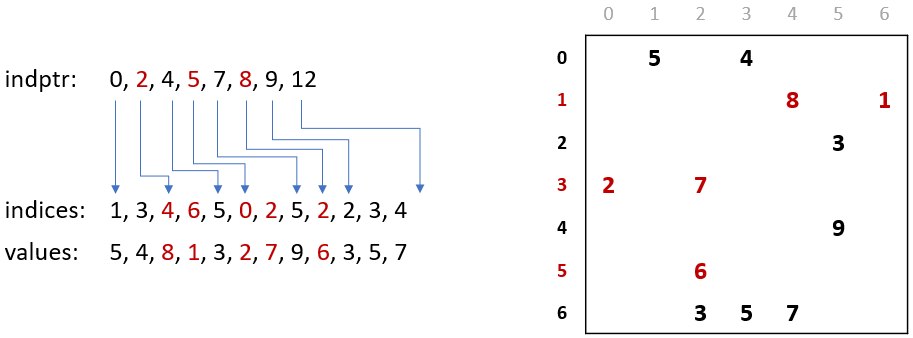
\includegraphics[width=4.5in]{GrB_CSR_FORMAT.png}
    \end{center}
    \caption{Data layout for CSR format.}
    \label{Fig:CSR_format}
    \hrule
\end{figure}

\subsection{{\sf GrB\_CSC\_FORMAT}}

The {\sf GrB\_CSC\_FORMAT} format indicates that a matrix will be imported or 
exported using the compressed sparse column (CSC) format.  {\sf indptr} is a 
pointer to an array of {\sf GrB\_Index} of size ncols+1 elements, where
the i'th index will contain the starting index in the {\sf values}
and {\sf indices} arrays corresponding to the i'th column of the matrix.
{\sf indices} is a pointer to an array of number of
stored elements (each a {\sf GrB\_Index}), where each element contains the 
corresponding element's row index within a column of the matrix.
{\sf values} is a pointer to an array of number of
stored elements (each the size of the scalar stored in the matrix) containing 
the corresponding value.  The 
elements of each column are not required to be sorted by row index.

\begin{figure}[h]
    \hrule
    \begin{center}
        ~\\
        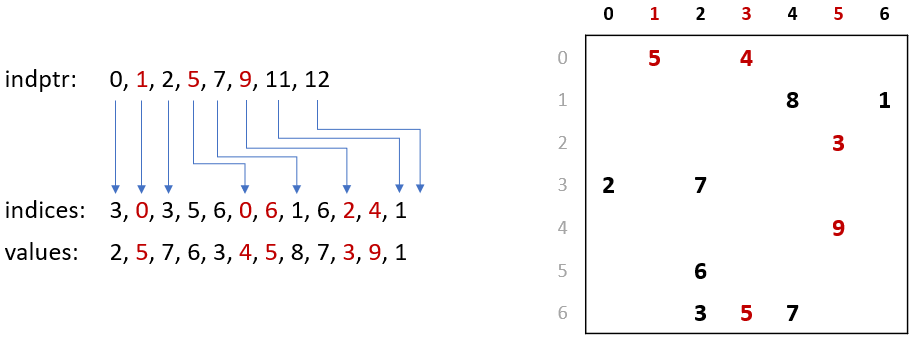
\includegraphics[width=4.5in]{GrB_CSC_FORMAT.png}
    \end{center}
    \vspace{-1em}
    \caption{Data layout for CSC format.}
    \label{Fig:CSC_format}
    \hrule
\end{figure}

\subsection{{\sf GrB\_COO\_FORMAT}}

The {\sf GrB\_COO\_FORMAT} format
indicates that a matrix will be imported or exported using the coordinate list
(COO) format.  {\sf indptr} is a pointer to an array of {\sf GrB\_Index} of size 
number of stored elements,
where each element contains the corresponding element's column index.
{\sf indices} will be a pointer to an array of {\sf GrB\_Index} of size 
number of stored elements, where each
element contains the corresponding element's row index.
{\sf values} will be a pointer to an array of size number of
stored elements (each the size of the scalar stored in the matrix) containing the corresponding value. Elements
are not required to be sorted in any order.

\begin{figure}[h]
    \hrule
    \begin{center}
        ~\\
        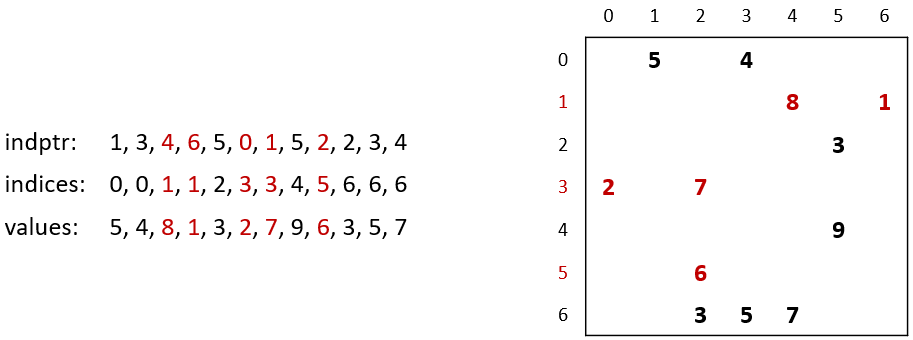
\includegraphics[width=4.5in]{GrB_COO_FORMAT.png}
    \end{center}
    \vspace{-1em}
    \caption{Data layout for COO format.}
    \label{Fig:COO_format}
    \hrule
\end{figure}

\comment{
\subsection{{\sf GrB\_DENSE\_ROW\_FORMAT}}

The {\sf GrB\_DENSE\_ROW\_FORMAT} format indicates that a matrix will be imported
or exported using the dense row-major format.  {\sf indptr} and {\sf indices} are unused,
and may be set to NULL, while {\sf values} will point to an array of size number of columns
times number of rows, where element i,j is located at index i*ncols + j. Elements will be
in the order they appear within each row, and rows will be in order.

\begin{figure}[h]
    \hrule
    \begin{center}
        ~\\
        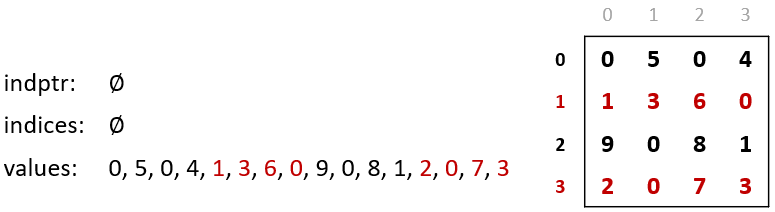
\includegraphics[width=4in]{GrB_DENSE_ROW_FORMAT.png}
    \end{center}
    \vspace{-1em}
    \caption{Data layout for the dense row-major format.}
    \label{Fig:DenseRow_format}
    \hrule
\end{figure}


\subsection{{\sf GrB\_DENSE\_COL\_FORMAT}}
The {\sf GrB\_DENSE\_COL\_FORMAT} format indicates that a matrix will be imported
or exported using the dense column-major format.  {\sf indptr} and {\sf indices} are unused,
and may be set to NULL, while {\sf values} will point to an array of size number of columns
times number of rows, where element i,j is located at index i + j*nrows. Elements will be
in the order they appear within each column, and columns will be in order.

\begin{figure}[h]
    \hrule
    \begin{center}
        ~\\
        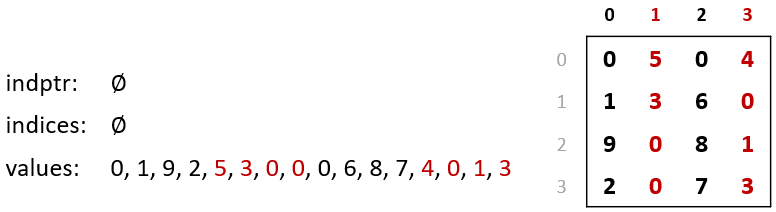
\includegraphics[width=4in]{GrB_DENSE_COLUMN_FORMAT.png}
    \end{center}
    \vspace{-1em}
    \caption{Data layout for the dense column-major format.}
    \label{Fig:DenseCol_format}
    \hrule
\end{figure}
}

%--------------------------------------------------------------
%--------------------------------------------------------------

\chapter{Examples}
\label{Chp:Examples}

\pagebreak
\nolinenumbers
\section{Example: level breadth-first search (BFS) in GraphBLAS}
{\scriptsize
\lstinputlisting[language=C,numbers=left]{BFS5M.c}
}
\vfill

\pagebreak
\nolinenumbers
\section{Example: level BFS in GraphBLAS using apply}
{\scriptsize
\lstinputlisting[language=C,numbers=left]{BFS6_apply.c}
}
\vfill

\pagebreak
\nolinenumbers
\section{Example: parent BFS in GraphBLAS}
{\scriptsize
\lstinputlisting[language=C,numbers=left]{BFS7_parents.c}
}
\vfill

\pagebreak
\nolinenumbers
\section{Example: betweenness centrality (BC) in GraphBLAS}
\label{App:BCnobatch}
{\scriptsize
\lstinputlisting[language=C,numbers=left]{BC1M_update.c}
}
\vfill

\pagebreak
\nolinenumbers
\section{Example: batched BC in GraphBLAS}
{\scriptsize
\lstinputlisting[language=C,escapechar=|,numbers=left]{BC1_batch.c}
}
\vfill

\pagebreak
\nolinenumbers
\section{Example: maximal independent set (MIS) in GraphBLAS}
{\scriptsize
\lstinputlisting[language=C,numbers=left]{MIS1.c}
}
\vfill

\pagebreak
\nolinenumbers
\section{Example: counting triangles in GraphBLAS}
{\scriptsize
\lstinputlisting[language=C,numbers=left]{TC1.c}
}
\vfill
\pagebreak

\linenumbers
